\section{Introduction}
In this laboratory session, the principles of interference and diffraction will be studied. Interference and diffraction are fundamental phenomena in wave optics, crucial for understanding light behavior. Interference occurs when waves overlap, resulting in either reinforcement or cancellation of amplitudes, generating distinctive patterns. Diffraction involves wave bending around obstacles or through narrow openings, producing diffraction patterns. By analyzing the resulting patterns, the wavelength of light can be deduced.

\begin{figure}[H]
    \centering
    \includegraphics{PHOTOS/Theorylab9.png}
    \caption{Phenomena of interference and Diffraction}
    \label{fig: theory}
\end{figure}

The theoretical framework includes the superposition principle for interference and the Fraunhofer diffraction equation:
\begin{equation} \label{eq: theory}
    d \cdot \sin(\theta) = d \cdot \frac{y}{\sqrt{y^2+x^2}} = m \cdot \lambda
\end{equation}
where $d$ is the slit spacing, $\theta$ is the diffraction angle, $m$ is the diffraction maximum, and $\lambda$ is the wavelength of light. Also, the sine is obtained by getting either the diffraction width or the slit width, depending on the pattern we are focusing on, and with the length from the observer. To make it easier, m=1 will be use, so only one calculation for the sin can be done with trigonometry. For its uncertainty, as derivated in homework:

\begin{equation} \label{eq: uncer}
    \sigma_\lambda =\lambda \cos{\theta}^2 \cdot \frac{\sigma_y}{y} =\lambda \left(\frac{x^2}{\sqrt{y^2+x^2}} \right)^2 \cdot \frac{\sigma_y}{y} 
\end{equation}

Additionally, the ratio of widths of the central diffraction peak to the central interference fringe is given by:
\[
\frac{2a}{b}
\]
where $a/b$ is the ratio of slit separation to slit width.

\subsection{Goals}
\vspace*{-2mm}
The objectives of this lab session are:
\vspace*{-2 mm}
\begin{itemize}
\item  Measure the wavelength of a laser with diffraction slit wheel.
\item  Measure the wavelength of a Hydrogen Lamp and a LED lamp with gratting lines diffractor.
\end{itemize}
\vspace*{-4 mm}
\section{Apparatus and procedure}
\vspace*{-4 mm}
\noindent The apparatus  use are:
\vspace*{-2 mm}
\begin{itemize}
    \item Ruler
    \item Diode laser (wavelength $\lambda = 650 \pm 10$ nm)
    \item Double slit pattern wheel with slit separation $a = 0.25 \pm 0.01$ mm and slit width $b = 0.040 \pm 0.005$ mm
    \item Screen for observing diffraction pattern
    \item Diffraction grating 600 lines/s
    \item Hydrogen lamp and LED sources
    \item Camera
\end{itemize}



\begin{figure}[H]
    \begin{minipage}[c]{.50\linewidth}
    Firstly, connect all the devices for experiment 1. This requires connecting the laser, and locating the diffraction slit wheel in the positions asked (a=0.04 and  d=0.25) so the laser is actually diffracted. Make sure that the beam goes thorough it. 

    \

    Turn off the lights, and see the results. Take measurements of the different spots that can be visualize and the lengths, or take a picture. If the last option was taken, then a software may be used to determine the requires length of the spots, as it was my case, so the code used to read the pixels of each photo is shown in the appendix: [\ref{code: const}].
    \end{minipage}
    \hfill
    \begin{minipage}[c]{.47\linewidth}
    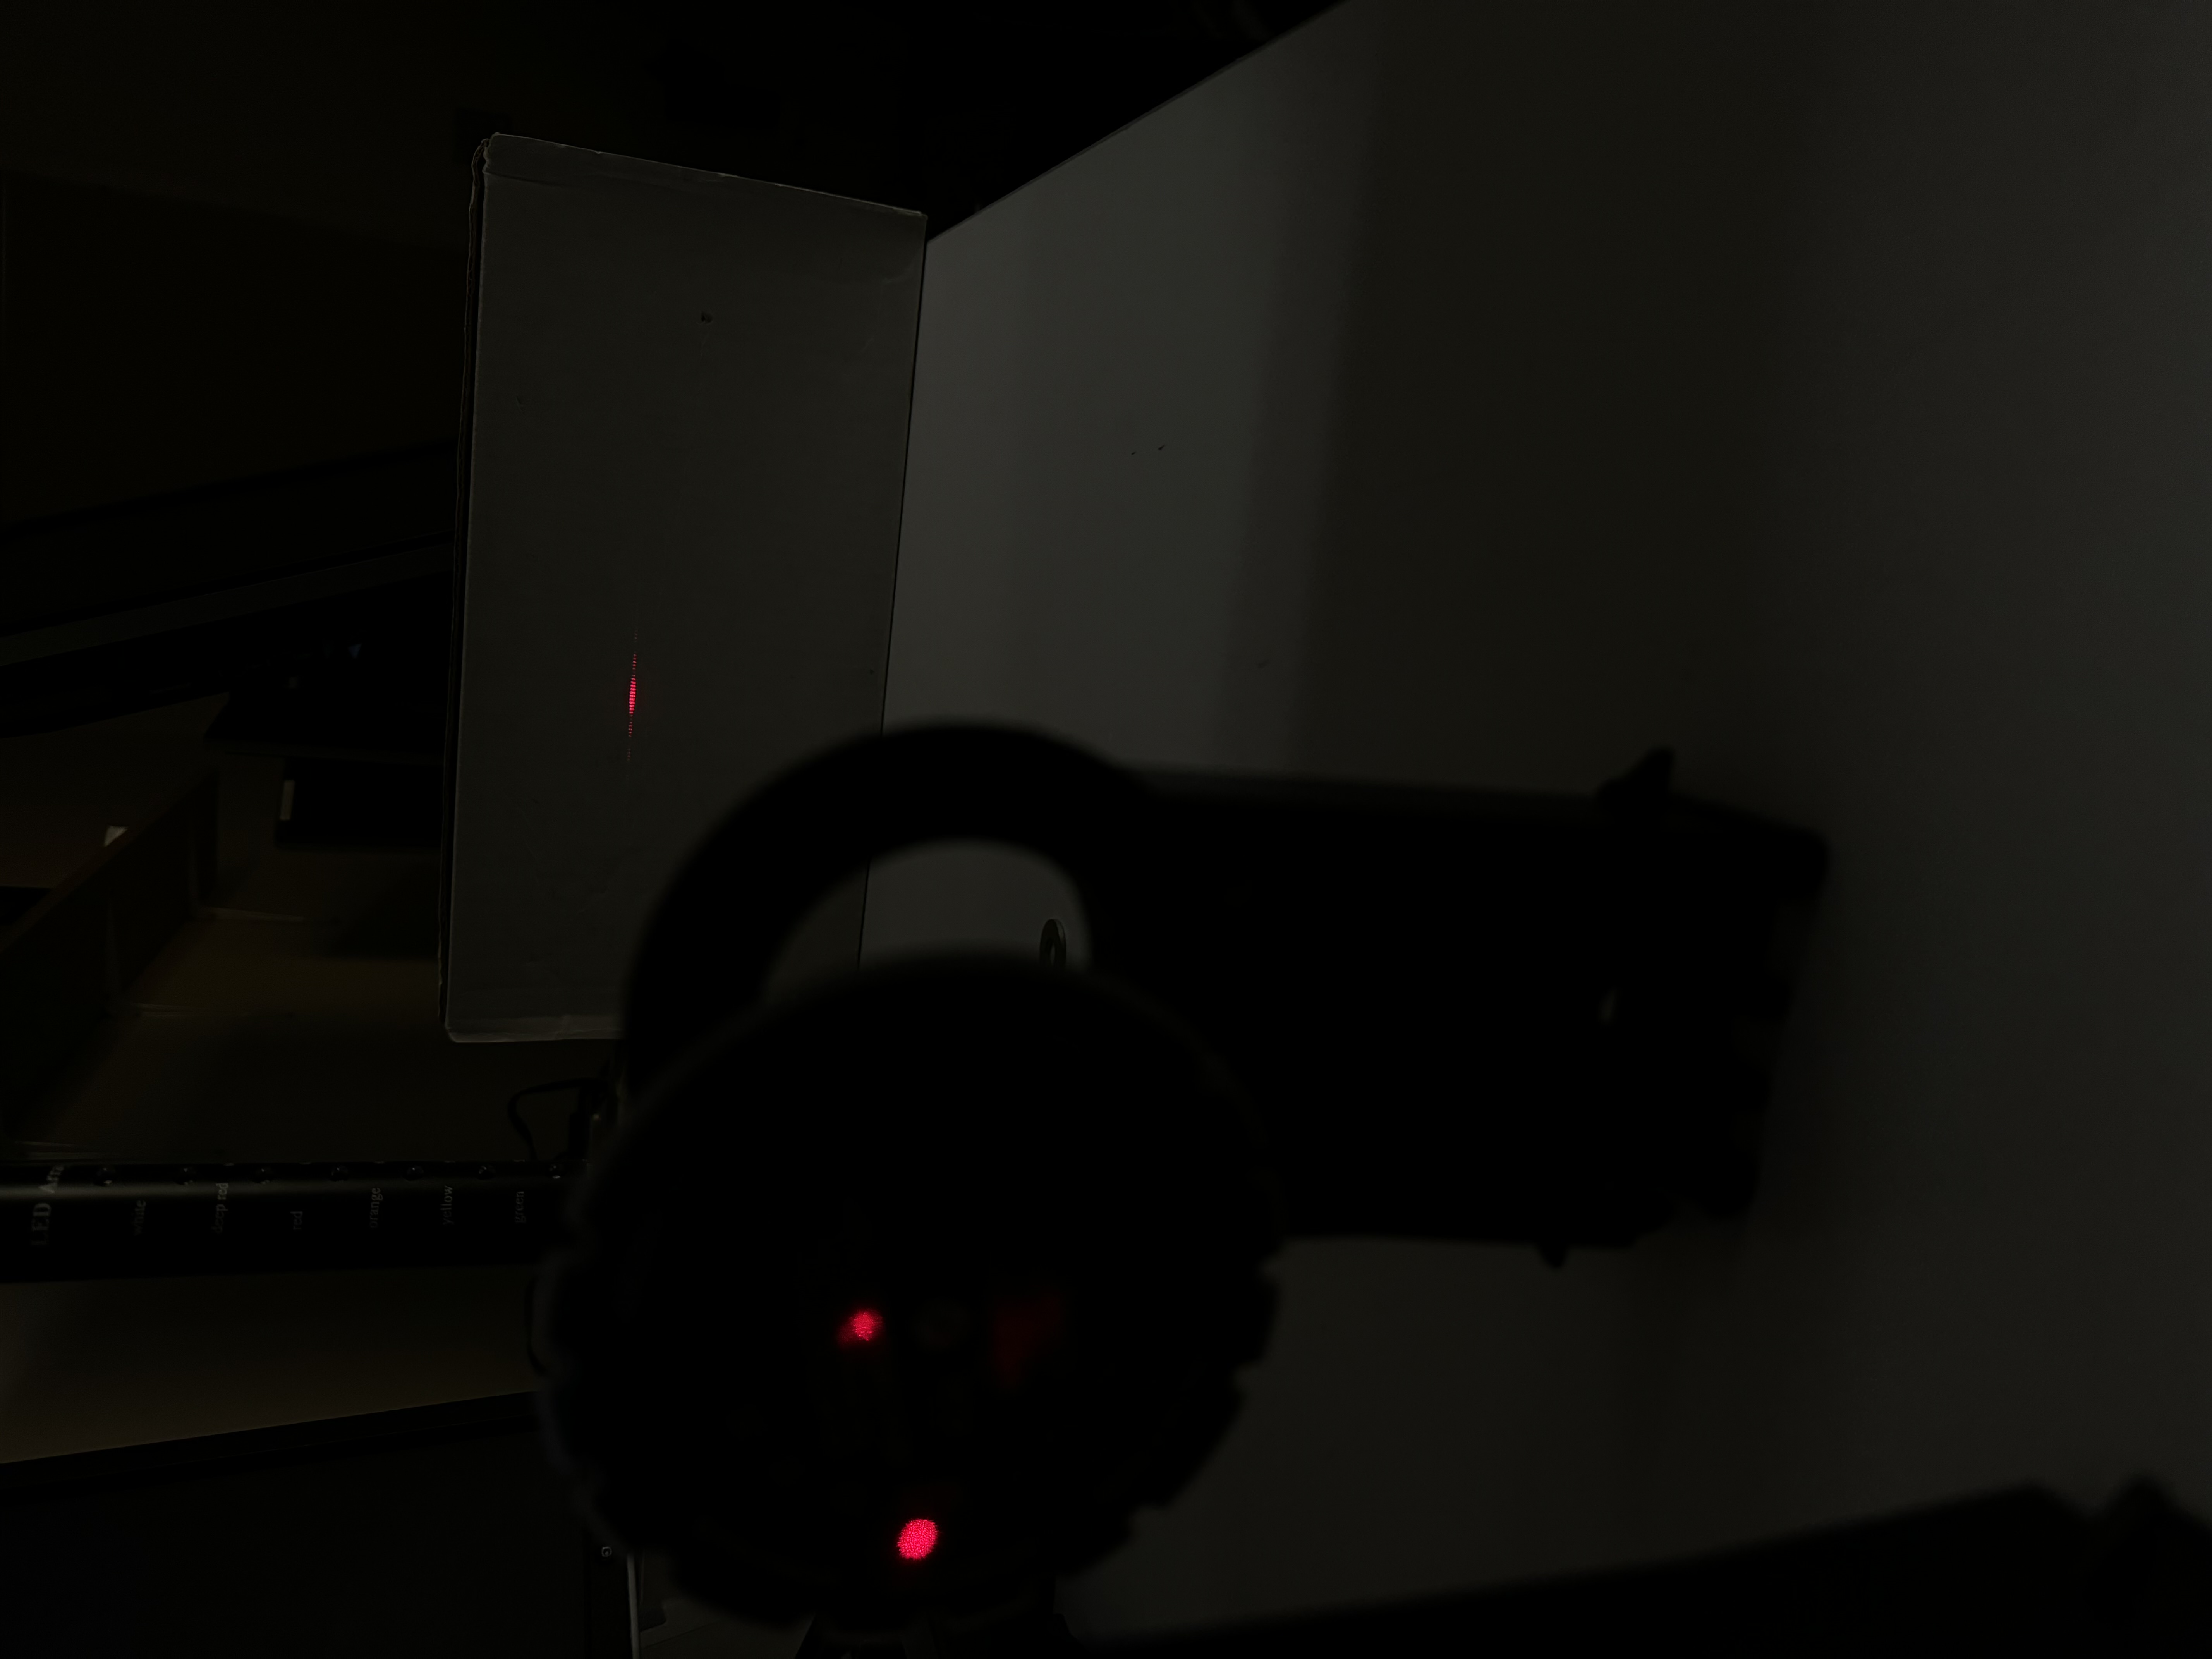
\includegraphics[width= 10 cm, rotate=-90]{PHOTOS/Setup_9.jpeg}
    \caption{Set-up first experiment}
    \label{fig: setup}
    \end{minipage}
\end{figure}


In the second experiment, the laser can be disconnected as a LED Lamp and a Hydrogen one will be used. And the same process should be done for both:
\begin{enumerate}
    \item Connect the Lamp
    \item Put the gratting layer on you eye
    \item Measure the distance between your eye and the lamp
    \item Measure the distance from the color lines that you can see with the layer, to the lamp, on both sides.
    \item Disconnect the lamp
\end{enumerate}

\section{Data}
\subsection{Experiment 1}

For this lab, I decided to take pictures as I was only one person, and the do the measurements with the pixels. The screen was 40 cm and in pixels in the photo [\ref{fig: zoom}] goes from x=1342 to x=3142, so the $\Delta x$=1800 pixels. Also, the distance away from the screen was 60 cm. In the following picture, it can be seen all the pictures:
\begin{figure}[H]
    \centering
    \includegraphics[width = 16 cm]{PHOTOS/whole pixels.png}
    \caption{Diffraction pattern using \ref{code: const}}
    \label{fig: diffpat}
\end{figure}
However, as it was difficult to measure from here, a zoom in was made in order to make it easier, and knowing also that the pixels will not change in the scale:
\begin{figure}[H]
    \centering
    \includegraphics[width = 15 cm]{PHOTOS/pixels.png}
    \caption{Zoom in for pixels measurements}
    \label{fig: zoom}
\end{figure}
Over 7 clear fringes can be observed in the photo. The first order fringe, which corresponded to the second brightest one of  interference, has a width of $\Delta\text{pixels}=$ 1946-1904 = 42, measured from fig [\ref{fig: zoom}]. The brightest one, that of the zero order, has a width of $a=\Delta\text{pixels}=$ 2030-1954 = 76 pixels among all its slits (10), and the diffraction one has a width of $b=\Delta \text{pixels}$ 1903-1892=11 pixels. 


\subsection{Experiment 2}
The Red LED had its lines: 88 cm and 5 cm, with and $x_0=46.5$, it was at 91 cm way from the observer. Then for the blue Led, the lines were at 76.5 cm and 16.5 cm at the same $x_0=46.5$, with a 98 cm length from the observer. 

For the Hydrogen Lamp, a photo was taken with the gratting, so the lines could be seen and then calculated thanks to the pixel conversion,  as seen in fig [\ref{fig: hydrogen}]. Looking into the figure, which is magnified, the results are that red lines have pixels at 3320 and 838, while light blue has it on 2960 and 1205. 
\begin{figure}[H]
    \centering
    \includegraphics[width = 17 cm]{PHOTOS/Hydrogen_Pixels.png}
    \caption{Hydrogen lines pictures using \ref{code: const}}
    \label{fig: hydrogen}
\end{figure}
The 0 for the ruler start at 615 pixel, and ends in the photo at 98 cm in 3528 pixels. The observer with the gratting lines was set at 94 cm from the lamp.

\section{Results}
\subsection{Experiment 1 }
\vspace*{-4 mm}
For the ratio of a/b, it can be directly calculated with the pixels, as they will suffer the same conversion to cm:
$$\frac{a}{b}=\frac{76}{11}\simeq6.9$$
And for the wavelength, we obtain that for the interference, which the difference from the first maxima and the zero value, using the pixels is 1987-1925=62 (a value), we get $62 \text{ pixels}\cdot \frac{40 \text{ cm}}{1800 \text{ pixels}} = 1.38$:
$$\sin{\theta}= \frac{y}{\sqrt{y^2+x^2}}= \frac{1.38}{\sqrt{1.38^2+80^2}}=0.017$$
From theory \eqref{eq: theory}, m=1:
$$\lambda = b \cdot \sin \theta = 0.04 \text{ mm}  \cdot 0.017 = \boxed{689.89 \ \text{nm}} $$
The uncertainty, as the ruler has an uncertainty of 1/2=0.5 mm. \eqref{eq: uncer}:
$$\sigma_\lambda = 689.89 \text{ nm} \left(\frac{80}{\sqrt{1.38^2+80^2}}\right)^2 \cdot \frac{0.5 \cdot 10^6}{1.38 \cdot 10^{7}} \text{mm} = \boxed{24.96 \ \text{nm}}$$


\subsection{Second Experiment}
The results for this experiments can be obtain by  knowing that a is obtained with the data of 600 lines/ mm, so $a=\dfrac{\mu m}{0.6}$.

And by taking the distance to it which was 91 cm in the RED LED, the distance from $x_0$ where at $\Delta x= |88-46.5| = |5-46.5|=41.5$ cm. 
$$\sin \theta = \frac{\Delta x}{\sqrt{(\Delta x)^2 + y^2}}= \frac{41.5}{41.5^2+91^2}$$
$$\lambda_\text{RedLED} = \sin \theta \cdot a = \frac{41.5}{41.5^2+91^2} \cdot \frac{1 \ \mu \text{m}}{0.6} = \boxed{691.15 \ nm} $$
For the Light Blue LED, distance from the observer was 94 cm, and the $\Delta x = 76.5-46.5= 30$ cm. So using the same formula:

$$\lambda_\text{BlueLED}  = \sin \theta \cdot a = \frac{30}{30^2+98^2} \cdot \frac{1 \ \mu \text{m}}{0.6} = \boxed{487.85 \ \text{nm}} $$
Now, for each uncertainty, using \eqref{eq: uncer}:
$$\sigma_{\lambda\text{RedLED}} =  6.89 \simeq 7 \text{ nm}$$
$$\sigma_{\lambda\text{BlueLED}}  = 7.4 \simeq 7 \text{ nm}$$

Now, for the Hydrogen Lamp, getting the distance from the pixels, we could fine that Red lines thanks to the conversion with the ruler and its measurements:
$$3320-615 \text{ pixels} \cdot  \frac{98 - 0 \text{cm}}{3528-615}= 3320 \cdot 0.0336 =  90.88 \text{ cm}$$
$$838-615 \text{ pixels} \cdot  \frac{98 - 0 \text{cm}}{3528-615}=  \cdot 0.0336 = 7.493 \text{ cm}$$
And the blue lines are find at:
$$2960-615 \text{ pixels} \cdot  \frac{98 - 0 \text{cm}}{3528-615}= 3320 \cdot 0.0336 =  78.79 \text{ cm}$$
$$1205-615 \text{ pixels} \cdot  \frac{98 - 0 \text{cm}}{3528-615}=  \cdot 0.0336 = 19.82 \text{ cm}$$

So using the formula for each, knowing that the initial problems is at 2075 pixels, which can be obtained following the above measure, so $X_0=$49.06. Hence, $\Delta x_\text{H Blue lines}= 78.79-49.06=29.73$ and $\Delta x_\text{H Red lines}= 90.88-49.06=41.82$  and we found that the lines are at:

$$\lambda_\text{H Blue}  = \sin \theta \cdot a = \frac{29.73}{29.73^2+94^2} \cdot \frac{1 \ \mu \text{m}}{0.6} = \boxed{502.589 \ \text{nm}} $$

$$\lambda_\text{H Red}  = \sin \theta \cdot a = \frac{41.82}{41.82^2+98^2} \cdot \frac{1 \ \mu \text{m}}{0.6} = \boxed{677.46 \ \text{nm}} $$
And their uncertainties, by using again the equation from theory:
$$\sigma_{\lambda\text{BlueLED}}  = 7.68 \simeq 8  \text{ nm}$$
$$\sigma_{\lambda\text{RedLED}} =  6.85 \simeq 7\text{ nm}$$

Putting all the information together, grabbing the empirical data from the lamps for LED and for Hydrogen from this source[\cite{guide}], and rounding the values with the last digit of the uncertainties.
\begin{table}[H]
\centering
\caption{Measured and expected values of wavelengths}
\begin{tabular}{lccc}
\toprule
Source & Measured value (nm) & Error (nm) & Expected Value (nm) \\
\midrule
Hydrogen - Blue & 450 & 8 & 434 \\
Hydrogen - Red & 680 & 7 & 656 \\
LED - Blue & 490 & 7 & 470 \\
LED - Red & 691 & 7 & 626 \\
\bottomrule
\end{tabular}
\end{table}

\section{Conclusions}

For the first experiment, the wavelength was determined to be $690 \pm 25$ nm, with the expected value being 650 nm, which was obtained from the guide. Doing the number of uncertainties:
$$\text{N of uncertainties}= \frac{|\lambda_{\text{exp}}- \lambda_{\text{theo}}|}{\sigma_\lambda}=\frac{690-650}{25}=1.6$$

As it is within the range of 2, we can determine that the result is good. However, one can notice the substantial uncertainty that the measurement has, and this came because they measurements have the order of 0.1 mm, or $10^5$ nm, which propagate into the wavelength uncertainty.

Regarding the ratio of the slit separation to the slit width, $\frac{a}{b}$, the theoretical value from the guide, one dividing both, is $6.25$. The measured value is $6.9$,  which is not pretty far from the expected one and may suggests that our measurements are consistent with the expected values. To study better the accuracy of it, an uncertainty should have been taken, but as in this part I was working only with pixels, the uncertainty was complicated to found.

In the second part of the experiment, to determine the accuracy we will do again the number of uncertainties found, a table will be done in order to have a better visualization:
\begin{table}[H]
\centering
\begin{tabular}{lcccc}
\toprule
Source & $\lambda_{\text{exp}}$ (nm) & $\sigma_\lambda$ (nm) & $\lambda_{\text{theo}}$ (nm) & N$^\circ$ of uncertainties \\
\midrule
Hydrogen - Blue & 450 & 8 & 434 & 2\\
Hydrogen - Red & 680 & 7 & 656 & 3.43 \\
LED - Blue & 490 & 7 & 470 & 2.86\\
LED - Red & 691 & 7 & 626 & 9.28\\
\bottomrule
\end{tabular}
\caption{Number of uncertainties}
\end{table}

From the Hydrogen Lamp, theoretical wavelengths for Blue and Red were determined. The measured value for Blue matches the theoretical value within 2 uncertainty, while Red surpass the limit. Thus, the results slightly accurate for the measurements taken, probably some propagation errors and human calculation may have affected. 

For the LEDs, theoretical wavelengths for Red and Blue were obtained and, the values does not match the theoretical values within the 2 uncertainties, actually, there RED Led had a really high one. Although, the uncertainties of the measurements were pretty straight along all this experiments, which means that the experiment itself was kind of precise, but as it does not match the number of uncertainties, meaning the not in agreement with the theory, it can be said that it was not accurate. 

All say, one should mention that also, errors where expected because not measuring everything by hand, and deciding which pixel was the most accurate one, if the photo was taken with the correct positions or if it was flattened because it has a little rotated... There were many different sources of errors that contributed to this result.



